%%%%%%%%%%%%%%%%%%%%%%% file template.tex %%%%%%%%%%%%%%%%%%%%%%%%%
%
% This is a general template file for the LaTeX package SVJour3
% for Springer journals.          Springer Heidelberg 2006/03/15
%
% Copy it to a new file with a new name and use it as the basis
% for your article. Delete % signs as needed.
%
% This template includes a few options for different layouts and
% content for various journals. Please consult a previous issue of
% your journal as needed.
%
%%%%%%%%%%%%%%%%%%%%%%%%%%%%%%%%%%%%%%%%%%%%%%%%%%%%%%%%%%%%%%%%%%%
%
% First comes an example EPS file -- just ignore it and
% proceed on the \documentclass line
% your LaTeX will extract the file if required
%\begin{filecontents*}{example.eps}
%!PS-Adobe-3.0 EPSF-3.0
%%BoundingBox: 19 19 221 221
%%CreationDate: Mon Sep 29 1997
%%Creator: programmed by hand (JK)
%%EndComments
%gsave
%newpath
%  20 20 moveto
%  20 220 lineto
%  220 220 lineto
%  220 20 lineto
%closepath
%2 setlinewidth
%gsave
%  .4 setgray fill
%grestore
%stroke
%grestore
%\end{filecontents*}
%
%\documentclass{svjour3}                     % onecolumn (standard format)
\documentclass[smallextended]{svjour3}     % onecolumn (second format)
%\documentclass[twocolumn]{svjour3}         % twocolumn
%
\smartqed  % flush right qed marks, e.g. at end of proof
%
\usepackage{graphicx}
%
\usepackage{mathptmx}      % use Times fonts if available on your TeX system
%
% insert here the call for the packages your document requires
%\usepackage{latexsym}
% etc.
\usepackage{subfig}
%
% please place your own definitions here and don't use \def but
% \newcommand{}{}
%
% Insert the name of "your journal" with
\journalname{Multibody System Dynamics}
%
\begin{document}

\title{Rider Motion Identification During Normal Bicycling by Means of Principal Component Analysis%\thanks{Grants or other notes
%about the article that should go on the front page should be
%placed here. General acknowledgments should be placed at the end of the article.}
}
%\subtitle{Do you have a subtitle?\\ If so, write it here}

%\titlerunning{Short form of title}        % if too long for running head

\author{Jason K. Moore \and
        J. D. G. Kooijman \and
	A. L. Schwab \and
	Mont Hubbard %etc.
}

%\authorrunning{Short form of author list} % if too long for running head

\institute{J. K. Moore and M. Hubbard \at
              Mechanical and Aerospace Engineering\\
	      University of California\\
	      One Shields Avenue, Davis, CA 95616-5294, USA\\
              Tel.: +01-530-752-0580\\
              Fax: +01-530-752-4158\\
              \email{jkmoor@ucdavis.edu, mhubbard@ucdavis.edu}           %  \\
%             \emph{Present address:} of F. Author  %  if needed
           \and
           J. D. G. Kooijman and A. L. Schwab \at
              Laboratory for Engineering Mechanics\\
	      Delft University of Technology
              Mekelweg 2, 2628 CD Delft, The Netherlands\\
              Tel.: +31 (0)15-27 85733\\
              Fax: +31 (0)15-27 82150\\
              \email{jodikooijman@gmail.com, a.l.schwab@tudelft.nl}
}

\date{Received: date / Accepted: date}
% The correct dates will be entered by the editor


\maketitle

\begin{abstract}
Recent observations of a bicyclist riding through town and on a treadmill show
that the rider uses the upper body very little when performing normal maneuvers
and that the bicyclist may in fact primarily use steering input for control.
They also revealed that other motions such as lateral movement of the knees
were used in low speed stabilization. In order to validate the hypothesis that
there is little upper body motion during casual cycling, an in-depth motion
capture analysis was performed on the bicycle and rider system.

We used motion capture technology to record the motion of three similar young
adult male riders riding two different city bicycles on a treadmill. Each rider
rode each bicycle while performing stability trials at speeds ranging from 2
km/h to 30 km/h: stabilizing while pedaling normally, stabilizing without
pedaling, line tracking while pedaling, and stabilizing with no-hands. These
tasks were chosen with the intent of examining differences in the kinematics at
various speeds, the effects of pedaling on the system, upper body control
motions and the differences in tracking and stabilization.

Principal component analysis was used to transform the data into a manageable
set organized by the variance associated with the principal components. In this
paper, these principal components were used to characterize various distinct
kinematic motions that occur during stabilization with and without pedaling.
These motions were grouped on the basis of correlation and conclusions were
drawn about which motions are candidates for stabilization related control
actions.
\keywords{bicycle \and principal component analysis \and motion capture \and human control}
% \PACS{PACS code1 \and PACS code2 \and more}
% \subclass{MSC code1 \and MSC code2 \and more}
\end{abstract}

\section{Introduction}
\label{intro}
Much progress has been made in understanding the rigid body dynamics of an
uncontrolled bicycle~\cite{Meijaard2007} and various control schemes have been
explored for tracking purposes~\cite{Peterson2008a,Schwab2008,Sharp2008a}, but
little is understood about how a bicyclist actually stabilizes a bicycle during
normal riding. A bicycle and rider system is unique among vehicles in the fact
that the rider is from 80 to 90 percent of the total mass of the system, the
system is laterally unstable and that the rider is flexibly coupled to the
bicycle in such a way that many body motions can be used as control inputs.
Previous research into realistic bicycle control has focused on both steering
and rider lean as control inputs, but there has been no experimental
verification of which motions a rider actually uses for control. Recent
observations of a bicyclist riding through town and on a
treadmill~\cite{Kooijman2009a} show that the rider moves the upper body very
little when performing normal maneuvers and that the bicyclist may in fact
primarily use steering input for control. This corresponds well with the fact
that control by leaning requires high gains compared to the gains required for
steering when employing a optimal control strategy on a model such as
LQR~\cite{Peterson2008a,Schwab2008,Sharp2008a}. The observations also revealed
that the rider may use other control inputs such as drastic knee movements at
low speeds. These conclusions were drawn by visually reviewing video data, so a
more rigorous objective method of characterizing the dominant movements of the
bicyclist while stabilizing a bicycle is needed. In order to validate the
hypothesis that there is little upper body motion during normal cycling, motion
capture techniques were used on the bicycle and rider system with the intent to
use principal component analysis to identify the major motion patterns.

Principal component analysis has successfully been used with data collected
from motion capture techniques to identify the dominant modes of motion of a
person walking on treadmill~\cite{Troje2002} and to characterize different
types of walking. We use similar methods for steady, normal bicycle riding on a
treadmill. Cyclic motions, such as pedaling, are easily identified and
separated from the other less cyclic control actions. Identifying the patterns
of movement gives insight into which body movements are primarily used and are
candidates for control inputs. This will be valuable for design of a realistic
biomechanical based control system of a bicycle rider, among other things.
\section{EXPERIMENTS}
\label{sec:exp}
To test our hypotheses, three riders performed a set of stability tasks in a
controlled environment while the motion of the bicycle and rider were collected
with a motion capture system. The tasks were performed on a $3\times5$ meter
treadmill Fig. (\ref{fig:treadmill}) capable of belt speeds up to 35 km/h. The
treadmill was chosen because the envelope of space was suitable for the motion
capture system and it eliminated any disturbances such as wind, rough ground,
and obstacles.  We chose three male riders of similar age [$27$ years
($\sigma=4$)] and build [height$=1.81$ m ($\sigma=0.04$) and mass$=73$ kg
($\sigma=1$)]. We also used two different Dutch bicycles: a 2008 Batavus
Browser with a 3 speed hub and a 2008 Batavus Stratos Deluxe with a 7 speed
hub. The Browser is described by the manufacturer as ``stable'' and the Stratos
Deluxe as ``nervous.''
\begin{figure}
    \centering
        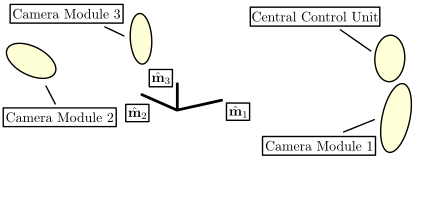
\includegraphics[width=\textwidth]{figures/treadmill.jpg}
    \caption{The $3\times5$ m treadmill at the Vrije Universiteit Amsterdam.}
    \label{fig:treadmill}
\end{figure}

We made use of the Optotrack Certus Motion Capture
System~\cite{NorthernDigitalIncorporated2009} to record the motion of the
bicycle and rider during the stability tasks. The system is based on active
infrared emitting markers that are placed on the moving bodies and connected to
a central control unit. Each marker emits an infrared signal at a different
frequency and the infrared pulses are captured by camera modules each
containing three cameras. The accuracy of the three dimensional measurements is
$\pm0.15$ mm. Wiring harnesses were built for both the rider and the bicycles
to facilitate easy bicycle and rider exchange Fig. (\ref{fig:markers}).
\begin{figure}
    \centering
        \subfloat[]{\label{fig:jodiBikeMarkers}\includegraphics[height=88mm]{figures/jodiBikeMarkers.pdf}}
        \subfloat[]{\label{fig:jodiMarkers}\includegraphics[height=88mm]{figures/jodiMarkers.pdf}}
    \caption{(a) Rider 1 and the Batavus Stratos Deluxe with marker positions. (b) Body marker positions visible from the rear.}
    \label{fig:markers}
\end{figure}

The marker coordinates were measured with respect to an inertial frame,
$\mathbf{M}$, where the plane normal to $\hat{\mathbf{m}}_3$ is coplanar with
the treadmill surface and $\hat{\mathbf{m}}_3$ is directed upward. We collected
the three dimensional locations of 31 markers, 11 of which were located on the
bicycle and 20 that mapped the rider Fig. (\ref{fig:markerloc}).
\begin{figure}
    \centering
        \includegraphics[width=80mm]{figures/markerLoc.pdf}
    \caption{Schematic of the marker positions. The bicycle and rider are colored light gray and dark gray, respectively.}
    \label{fig:markerloc}
\end{figure}

The markers were placed on the bicycle so that we could easily extract the
rigid body motion (i.e. body orientations and locations) of the bicycle frame
and fork. Four markers were attached to the fork and seven markers were
attached to the rear frame. A marker was attached on the right and left sides
of the center of each wheel, the seat stays, the ends of the handlebars, and
the head tube. A single marker was also attached to the back of the seat post.

We recorded the location of 20 points on the rider: left and right sides of the
helmet, back of the helmet, shoulders, elbows, wrists, between the shoulder
blades on the spine, the midpoint between the shoulder blades and the coccyx,
the coccyx, hips, knees, ankles and feet. The body markers were not placed such
that a complete rigid body model could easily be fit to the data. This was done
to save setup and processing time because we only wanted a stick figure
representation of the rider that allowed us to visually observe the dominant
motions of the rider.

The stability tasks were designed such that the rider rode at a constant speed
within the range of 2 to 30 km/h. The bicyclists were told to maintain an
upright straight ahead course on the treadmill and to look into the distance,
with exception of the line tracking task. The bicyclists were instructed to
bicycle comfortably at the designated speed and the data recording was started
at random. In all cases the subject rode at the set speed until comfortable,
then data was taken for 60 seconds at a 100 hertz sampling rate. Each test was
performed on each bicycle with each rider. The following list gives the various
tests and their descriptions:

\begin{description}[Without pedaling]
 \item[Normal pedaling] The subject was instructed to simply stabilize the
     bicycle while pedaling and keep the heading in approximately the forward
     direction. The speed started at 5 km/h and increased in 5 km/h increments
     up to 30 km/h. The speeds were then decreased in the same fashion to 5
     km/h. From then on the speed was decreased in 1 km/h increments until the
     subject was not able stabilize the bicycle any longer. Therefore, there
     were two sets of data for each speed and each bicycle except speeds below
     5 km/h. Several additional runs were also performed with the rider
     pedaling using a different gear and thus a different cadence.
 \item[Without pedaling] This was the same as the normal pedaling task except
     that a string was attached to the head tube of the bicycle such that the
     bicycle was fixed longitudinally relative to the treadmill and no pedaling
     was required. The rider kept the feet in the same position throughout the
     task.
 \item[No-hands] The rider stabilized the bicycle without using steering for
     control. They were instructed to keep their hands on their hips while
     bicycling. The rider started at 30 km/h and decreased in 5 km/h increments
     through 20 km/h and thereafter the speeds were decreased in 1 or 2 km/h
     increments until the rider was not able to comfortably stabilize the
     bicycle.
 \item[Line tracking] This was the same as normal pedaling except that the
     rider was instructed to track a line on the treadmill surface with the
     front wheel. A smaller subset of speeds was performed.
\end{description}
These tasks were designed with the intent to answer several questions:
\begin{enumerate}
    \item What upper body motions are used while bicycling?
    \item How does the motion of the system change with respect to change in forward speed?
    \item How much does pedaling influence the control actions?
    \item Can the open loop rigid body dynamics be detected in the controlled state?
    \item What does the rider do differently to control the bicycle when riding no-hands?
    \item Do different bicyclists perform similar motions while performing the same task?
    \item Is there a difference in motion when stabilizing and trying to track a line?
\end{enumerate}
Since there is no room to address all of these questions in this paper, we
focus on a single rider on the Browser bicycle and two of the tasks: normal
pedaling and without pedaling. We were able to draw some conclusions on
questions 1 through 4 with this smaller data set.

\section{Open loop rigid body dynamics}
\label{sec:openLoop}
One question we have is whether or not the eigenfrequencies of the weave motion
for the uncontrolled system can be detected in the results from the
stabilization tasks. In order to predict the uncontrolled (open loop)
eigenvalues of the rigid rider system, the basic geometry, mass, center of
gravity locations, and moments of inertia of the bicycle were measured. Also,
the riders were measured and weighed such that the body segment geometry, mass,
center of gravity locations, and moments of inertia could be estimated. These
methods are described in \cite{Moore2009a}. This data was used to calculate
eigenvalues and eigenvectors of the uncontrolled open loop system Fig.
(\ref{fig:eigPlot}).
\begin{figure}[]
    \begin{center}
        \includegraphics[width=\textwidth]{figures/eigPlot.pdf}
    \end{center}
    \caption{Eigenvalues of the Browser bicycle with the third rider as a
    function of speed. Note that the initially unstable weave motion becomes
    stable above 16 km/h, the weave speed.}
    \label{fig:eigPlot}
\end{figure}

\section{Data processing}
\label{sec:data}

\subsection{Missing markers}
\label{sec:missingMarkers}
The Optotrack Certus Motion Capture
System~\cite{NorthernDigitalIncorporated2009} is based on the cameras' ability
to detect the infrared light from the sensors so there are occasional gaps in
the coordinate data due to the markers going out of view. We attempted to
minimize this by careful marker and camera placement but were not able to
totally eliminate the error. Any missing markers on the bicycle were
reconstructed using the fact that the bicycle is a rigid body. We had more than
three markers on both the frame and fork, so if one marker location was not
detected we used the relative location of the remaining markers to reconstruct
the missing marker. The gaps in the data of the markers on the human were
repaired by fitting a cubic spline through the data. The spline estimated the
marker coordinates during the gaps. We only used the splined data if the gaps
were less than 10 time steps, or 0.1 sec, otherwise the trials were discarded.

\subsection{Relative motion}
\label{sec:relativeMotion}
We were interested in the analysis of three different marker combinations: the
bicycle, the rider and the bicycle/rider. The motion of the bicycle and the
bicycle/rider were calculated with reference to the $\mathbf{N}$ inertial frame
and the motion of the rider was calculated with respect to the rear frame of
the bicycle $\mathbf{B}$ Fig. (\ref{fig:frames}). These three marker
combinations allowed us to differentiate more easily between rider specific and
bicycle specific motions. Furthermore, six of the variables that describe the
configuration of the bicycle in time were calculated to give insight into the
rigid body dynamics. Details of these calculations are shown in
Appendix~\ref{sec:inFrames}.
\begin{figure}[]
    \begin{center}
        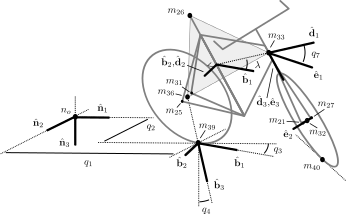
\includegraphics[width=\textwidth]{figures/frames.pdf}
    \end{center}
    \caption{Diagram of the bicycle's inertial frame $\mathbf{N}$, rear frame $\mathbf{B}$, front frame $\mathbf{E}$ and configuration variables.}
    \label{fig:frames}
\end{figure}

\subsection{Principal Component Analysis}
\label{sec:pca}
We used Principal Component Analysis~\cite{Jolliffe2002} to extract and
characterize the dominant motions of the system. Calculating the principal
components effectively transforms the space of the data to a space that
maximizes the variance of the data. The typical advantage of PCA is that the
dimension of the system can be reduced and still retain enough information to
adequately describe the system. We are primarily interested in the way that PCA
is able to extract linear components and rank them in order of variance from
the mean position. If we assume that the components with the largest kinematic
variance are motions that are the dominant motions used for control and
propulsion (which in general is not necessarily true for dynamical systems) the
comparison of these components for different riding conditions can give insight
into what motions may be important for developing a biomechanical control model
of the bicyclist.

The repaired data from the motion capture measurements contained the $x$, $y$,
and $z$ coordinates of each marker $1$ through $l$ at each time step $j=1$,
$2$, $\ldots$, $n$. Each marker has three coordinates so there are a total of
$m=3l$ coordinates $i=1$, $2$, $\ldots$, $m$. The coordinates at each time step
can be collected in vector $\mathbf{p}_j$.
\begin{displaymath}
    \mathbf{p}_j^T=\left[x_{1j}\quad\ldots\quad x_{lj}\quad y_{1j}\quad\ldots\quad y_{lj}\quad z_{1j}\quad\ldots\quad z_{lj}\right]=\left[p_{1j}\quad p_{2n}\quad\ldots\quad    p_{mj}\right]
\end{displaymath}
We can organize these coordinate vectors into a matrix, $\mathbf{P}$, where the
rows, $i$, map a single coordinate of a marker through $n$ time steps.
\begin{displaymath}
\mathbf{P}=\left[ \begin{array}{cccccc}
|              & |              &        & |              &        & |             \\
\mathbf{p}_{1} & \mathbf{p}_{2} & \ldots & \mathbf{p}_{j} & \ldots & \mathbf{p}_{n}\\
|              & |              &        & |              &        & |
\end{array} \right]
\end{displaymath}

The principal components were calculated for the three marker combinations as
described earlier where $n=60\cdot100=6000$ time steps. The number of rows of
$\mathbf{P}$ were ($m=3\cdot31=93$), ($m=3\cdot11=33$) and ($m=3\cdot21=63$)
for the bicycle/rider, the bicycle alone and the rider alone, respectively.

One method of determining the principal components is to calculate the
eigenvectors of the covariance matrix of the mean-subtracted data. We begin by
calculating the mean Eq. (\ref{eq:mean}) of the rows of $\mathbf{P}$ and
subtracting it from each column of $\mathbf{P}$ to form the mean-subtracted
data matrix $\mathbf{B}$ Eq. (\ref{eq:B}).
\begin{equation}
    \mathbf{u}=\frac{1}{n}\sum_{j=1}^n\mathbf{p}_j
    \label{eq:mean}
\end{equation}
A vector of ones
\begin{displaymath}
    \mathbf{h}^T=\left[h_1\quad h_2\quad\ldots\quad h_j\quad\ldots\quad h_n\right]\textrm{ where }h_j=1\textrm{ for all }j
    \label{eq:h}
\end{displaymath}
allows us to subtract $\mathbf{u}$ from each column of $\mathbf{P}$,
\begin{equation}
    \mathbf{B}=\mathbf{P}-\mathbf{u}\mathbf{h}^T
    \label{eq:B}
\end{equation}
The covariance matrix $\mathbf{C}$ of $\mathbf{B}$ can then be calculated with
Eq. (\ref{eq:C}).
\begin{equation}
    \mathbf{C}=\frac{1}{n-1}\mathbf{B}{\mathbf{B}^T}
    \label{eq:C}
\end{equation}
Calculating the eigenvectors $\mathbf{v}_i$ and eigenvalues $\lambda_i$ of the
covariance matrix effectively transforms the space to one where the variances
are maximized and the covariances are zero. The eigenvectors are the principal
components of the data set and the corresponding eigenvalues represent the
variance of each principal component. The eigenvectors are ordered by
decreasing eigenvalue where $\mathbf{v}_1$ is the eigenvector corresponding to
the largest eigenvalue. The eigenvalues and eigenvectors are calculated by
finding the independent solutions to Eq. (\ref{eq:eig}).
\begin{equation}
    \mathbf{C}\mathbf{v}_i=\lambda_i\mathbf{v}_i
    \label{eq:eig}
\end{equation}
Each time step can now be represented as a linear combination of the principal
components.
\begin{equation}
    \mathbf{p}_j=\mathbf{u}+a_{1j}\mathbf{v}_1+a_{2j}\mathbf{v}_2+\ldots+a_{mj}\mathbf{v}_m
    \label{eq:linComb}
\end{equation}
The coefficients $a_{ij}$ can be solved for each time step $j$ by reformulating
Eq. (\ref{eq:linComb}) and solving the system of linear equations.
\begin{equation}
    \mathbf{P}-\mathbf{u}\mathbf{h}^T=
    \left[\begin{array}{cccc}
        | & | & & |\\
        \mathbf{v}_1 & \mathbf{v}_2 & \ldots & \mathbf{v}_m\\
        | & | & & |
    \end{array}\right]
    \left[\begin{array}{ccc}
    a_{11} & \ldots & a_{1n}\\
    \vdots & \ddots & \vdots\\
    a_{m1} & \ldots & a_{mn}
    \end{array}\right]
    =\mathbf{V}\mathbf{A}
\end{equation}
and
\begin{equation}
    \mathbf{A}=\mathbf{V}^{-1}(\mathbf{P}-\mathbf{u}\mathbf{h}^T)\textrm{.}
\end{equation}
With the principal components $\mathbf{v}_i$ being constant, the behavior in
time is described by the coefficients $a_{ij}$ where the discretization in time
is indexed by $j$. The order of the system can be reduced by eliminating
principal components that have little variance. We arbitrarily decided to
examine the first $k=10$ principal components knowing that the first five would
be based around the larger motions such as pedaling and that the remaining five
may reveal some of the motions associated with control. The variance of each
component, $\textrm{var}(\mathbf{a}_i)=\lambda_i$, is summed to determine the
cumulative percentage of variance of the principal components, $g_k$.
\begin{equation}
    g_k=100\frac{\sum_{i=1}^k\lambda_i}{\sum_{i=1}^m\lambda_i}\textrm{ where }1\leq k\leq m
\end{equation}
Highly correlated data will show that even when $k<<m$, $g_k$ is close to
100\%. Using 10 components $g_{10}$ covers 100\% ($\sigma=2\cdot10^{-14}$\%) of
the variation in the data for the bicycle, rider and bicycle/rider. The matrix
$\mathbf{A}$ can then be reduced to a $k\times n$ matrix and eigenvectors
greater than $\mathbf{v}_k$ can be eliminated.

\subsection{Data Visualization}
\label{sec:dataVis}
We developed a graphical user interface in \textsc{Matlab} that easily allows
different trials to be compared with one another Fig. (\ref{fig:GUI}). The
program loads in two different trials along with information on the trial. A
graphical representation of the rider and bicycle are displayed in two adjacent
screens and can be viewed from multiple perspectives. The animations of the
runs can be played at different speeds, rewound and fast forwarded. The
principal components are shown beside the corresponding animation display and
combinations can be turned on and off for identification and comparison.
Frequency and amplitude information for the temporal coefficients $a_{ij}$ can
also be displayed for comparison.
\begin{figure}[]
    \begin{center}
        \includegraphics[width=\textwidth]{figures/GUI.pdf}
    \end{center}
    \caption{Screen shot of the \textsc{Matlab} graphical user interface (GUI) used to visualize principal components and compare between different components and trials.}
    \label{fig:GUI}
\end{figure}

\section{Results}
\label{sec:results}
\subsection{Motion identification}
\label{sec:motionId}
The reduced set of data provides two important pieces of information for the
identification of motion: the principal components $\mathbf{v}_i$ and the
corresponding coefficients $a_{ij}$. The principal components represent linear
trajectories of the markers and the coefficients show how the markers follow
the trajectories with time. We began processing the data by reviewing each
principal component of each trial in the GUI and noting down what type of
motion we saw Tab. (\ref{tab:trialDesc}). These descriptions were subjective
because we grouped marker movement based on our preconceived understanding of
rider and bicycle motion. Some of the modes displayed motions that were not
physically possible such as the upper leg stretching in length during the knee
bounce. This is possible when examining a single component but when
superimposed over the rest of the components the unrealistic motions are not
present. Furthermore, for each component we examined amplitude and frequency
content of the associated coefficients $a_{ij}$ as shown in Fig.
(\ref{fig:3062}) and noted down the shape of the frequency spectrum and the
frequencies at any distinct spikes.

\begin{table}
    \caption{Example raw trial description for the bicycle and rider during normal pedaling at 10 km/h.}
    \label{tab:trialDesc}
    \centering
    {\small
	\begin{tabular}{rrp{40mm}p{40mm}}
	\hline\noalign{\smallskip}
        $i$ & \% Variance & Motion Description & Frequency Description\\
        \noalign{\smallskip}\hline\noalign{\smallskip}
        1  & 45.50 & primarily longitudinal motion, some lateral & max amp=0.6m, most freq below 0.5hz, tiny spike at 1.6hz\\
        2  & 29.39 & primarily lateral motion, some longitudinal, small feet motion & little spike at 0.8hz, max amp=0.35m, most freq below 0.5hz\\
        3  & 15.41 & vertical pedaling, slight spine bend, hip/head/shoulder sway out of phase with pedaling & large dominant spike at 0.8hz, max amp=0.27m\\
        4  & 8.27  & horizontal pedaling, head/shoulder sway & large dominant spike at 0.8hz with 0.19m amp\\
        5  & 0.82  & yaw, knees stay still & most freq below 1hz, spike at 0.33hz and 0.04m\\
        6  & 0.27  & erratic left hand movement & max amp=0.018hz, most freq. below 2hz\\
        7  & 0.21  & steer, left hand movement, slight roll & most freq below 2hz, spike at 0.33hz and 1.58hz\\
        8  & 0.07  & knee and head bounce & dominant spike at 1.58hz\\
        9  & 0.04  & lat knee movement, head jiggle & spikes at 1.58hz and 2.37hz, most freq below 2.5hz\\
        10 & 0.02  & head and knee jiggle & spikes at 1.58hz and 3.17hz, most freq below 3.5hz\\
	\noalign{\smallskip}\hline
        \end{tabular}
    }

\end{table}

\begin{figure}[tb]
    \begin{center}
        \subfloat[]{\label{fig:coef3062}\includegraphics[width=0.5\textwidth]{figures/coef3062.pdf}}
        \subfloat[]{\label{fig:fft3062}\includegraphics[width=0.5\textwidth]{figures/fft3062.pdf}}
    \end{center}
    \caption{(a) Coefficients $a_{ij}$ versus time and (b) the frequency
    content of the first five principal components for normal pedaling at 10
    km/h. The vertical line in (b) represents the open loop weave frequency
    (0.28hz) determined from Fig. (\ref{fig:eigPlot}) at this forward speed .}
    \label{fig:3062}
\end{figure}
Several conclusions can be drawn from examining the coefficient data. First of
all, some of the components are linked by the frequencies of the coefficients
and describe an identifiable motion. The most obvious being that the vertical
and horizontal pedaling components make up the circular pedaling motion. They
both vary periodically and have a dominant frequency which is defined by the
cadence. In the example trial, Tab. (\ref{tab:trialDesc}), the upper body
motions are also linked to the pedaling. Components 8 and 9 are both based
around a frequency that is twice the pedaling frequency which may be due to the
forces created at each pedal stroke. Component 6 seems to be the result of a
bad marker signal. Components 5 and 7 are interesting because they display
motions of the bicycle that are not dominated by the pedaling frequency and may
be candidate control motions. The percentage variance of each component gives
an idea of the relative amplitude of the components. The descriptions of each
trial were used to compile a list of motions that contribute to the principal
components. These motions, illustrated in Fig. (\ref{fig:motions}), are:
\begin{description}[Pedaling]
    \item[Drift] The bicycle and rider drift longitudinally and laterally on
        the surface of the treadmill. The motions are typically defined by two
        components that are not necessarily orthogonal or aligned with the
        inertial coordinate system. The motion is random and at low
        frequencies.
    \item[Steer] Rotation of the front assembly with respect to the rear frame.
        The steering may appear linked to one of the pedaling components at the
        pedaling frequency or may be in one or more components sometimes
        combined with roll and/or yaw at more random frequencies, Fig.
        (\ref{fig:steerRoll}).
    \item[Roll] The bicycle and the rider roll with respect to the ground
        plane. Roll is typically linked with steer and/or yaw and often at the
        pedaling frequency, Fig. (\ref{fig:steerRoll}).
    \item[Yaw] The heading angle of the bicycle and rider change together with
        respect to the ground plane. This is typically linked with steer, roll
        and/or the drift, Fig. (\ref{fig:yaw}).
    \item[Pedaling] This motion is defined by two or more components, typically
        a vertical and horizontal motion of the feet, that show the feet
        rotating around the crank axle at a distinct frequency and the legs
        following suit, Fig. (\ref{fig:pedaling}).
    \item[Bend] The spine bent laterally and was always connected with the
        vertical pedaling component, Fig. (\ref{fig:bend}).
    \item[Lean] The upper body, shoulders and head lean laterally with respect
        to the rear frame and was always linked with the horizontal pedaling
        component, Fig. (\ref{fig:lean}).
    \item[Twist] The shoulders rotate about the torso axis. This was linked to
        components that contained steering motions both random and at the
        pedaling frequency, Fig. (\ref{fig:twist}).
    \item[Bounce] The knee markers bounce up and down, the back straightens and
        the head nods at twice the pedaling frequency, Fig.
        (\ref{fig:bounce}).
    \item[Knees] The knees move laterally relative to the bicycle frame in both
        opposing directions and the same direction at random low frequencies,
        Fig. (\ref{fig:knees}).
    \item[Head] Head twists and random head motions showed up often. These
        seemed to be due to the rider looking around randomly.
\end{description}
\begin{figure}[]
    \begin{center}
        \subfloat[]{\label{fig:steerRoll}\includegraphics[width=25mm]{figures/rollSteer.pdf}}\qquad
        \subfloat[]{\label{fig:yaw}\includegraphics[width=25mm]{figures/yaw.pdf}}\qquad
        \subfloat[]{\label{fig:pedaling}\includegraphics[width=25mm]{figures/pedal.pdf}}\qquad
        \subfloat[]{\label{fig:bend}\includegraphics[width=25mm]{figures/bend.pdf}}

        \subfloat[]{\label{fig:lean}\includegraphics[width=25mm]{figures/lean.pdf}}\qquad
        \subfloat[]{\label{fig:twist}\includegraphics[width=25mm]{figures/twist.pdf}}\qquad
        \subfloat[]{\label{fig:bounce}\includegraphics[width=25mm]{figures/bounce.pdf}}\qquad
        \subfloat[]{\label{fig:knees}\includegraphics[width=25mm]{figures/knees.pdf}}
    \end{center}
    \caption{Diagrams of the common motions. (a) Top view of the bicycle steer
    and roll, (b) the bicycle yaw, (c) the horizontal and vertical components
    of pedaling, (d) the spine bend, (e) rider lean, (f) top view of the rider
    twist, (g) knee bounce and (h) two knee motions. All but the pedaling are
    exaggerated for clarity.}
    \label{fig:motions}
\end{figure}

\subsection{Motion Characterization}
\label{sec:motionChar}
To identify how bicycling changes with speed it would be ideal to investigate
how the amplitude of each component varies with speed. However as the analysis
does not return the same set of components for each run such a comparison is
typically not possible. Therefore components were grouped into classes, where
each class shows a specific physically relevant motion. The same total motion
of the class can be described by one set of components in one trial and
another, probably different, set of components in another trial. How the
amplitudes of these classes change between two experiments can be used as a
measure for how bicycling has changed among trials.

To objectively identify which coefficients show the same type of motion and
could therefore form a class, the frequency content of each of the time
coefficients in a single trial was correlated to that of each of the other
components in that trial. Next a minimum correlation value was set to determine
which coefficients were correlated to each other. When the minimum was set at
0.9 only the coefficients making up the pedaling motion could be considered
correlated. On the other hand when a minimum level of 0.7 was used practically
every coefficient was correlated to each other. The only exception was the
coefficient that displayed the bounce. Its maximum correlation with another
coefficient was no higher than 0.4 for any of the tested speeds. The 0.8 level
gave a number of distinct classes of components and thus this level was used to
identify which coefficients were connected. Finally, the correlated
coefficients were viewed simultaneously in the GUI enabling the determination
of the motion class.

The correlated coefficients were used to form six different classes of motions,
each made up of combinations of the previously described motions, with
reference to Fig. (\ref{fig:motions}):
\begin{description}[Steer-Yaw-Roll]
    \item[Drift] Drift.
    \item[Pedaling] Pedaling (\ref{fig:pedaling}), Bend (\ref{fig:bend}), Lean (\ref{fig:lean}), Twist (\ref{fig:twist}).
    \item[Steer-Yaw-Roll] Steer and Roll (\ref{fig:steerRoll}), Yaw (\ref{fig:yaw}).
    \item[Bounce] Bounce (\ref{fig:bounce}).
    \item[Knees] Knees (\ref{fig:knees}).
    \item[Others] Head and components that showed noise of some
    sort.
\end{description}

In most cases the correlated coefficients described a single class. However, in
some cases this was not the case and the coefficients were used to describe
more than one class. An example is that at low speed the components containing
the drift motions also contained large steer, yaw and roll motions. Therefore,
the motions were placed in both the Drift and the Steer-Yaw-Roll classes.

Since the rider was not instructed to hold a specific location on the treadmill
the Drift class, which was usually the class with the largest amplitude, was
not used in further analysis of the motion and neither was the `Other' class.
For each of the remaining classes, the percentages of variance of the remaining
components were recalculated without the components placed in the Drift and the
Other classes.

By transforming the bicycle marker locations into rigid body motions for the
bicycle (See Appendix \ref{sec:inFrames}) it was also possible to investigate
the bicycle lean, yaw and steering motions. By carrying out a Fourier transform
these bicycle motions could also be investigated in the frequency domain.

\subsection{Characterization of motions during normal pedaling}
\label{sec:normalPed}
Figure (\ref{jellybean}) shows how the percentage of the four classes:
Pedaling, Steer-Yaw-Roll, Bounce and Knees vary with speed. From the graph it
is clear that at 10 km/h and higher speeds practically all the motion that is
taking place is the pedaling motion class. Below 10 km/h, the Steer-Yaw-Roll
class becomes increasingly active and the relative percentage of the motion
taking place in the pedaling class drops. Also at speeds below 10 km/h the
lateral knee motion (Knees) class percentage increases with decreasing speed.
The increase is not as significant as that of the Steer-Yaw-Roll class
(increase to roughly 5\% at 2 km/h), but it is certainly visible. The Bounce
roughly remains constant at all speeds.
\begin{figure}[]
    \centering
    \includegraphics[width=\textwidth]{figures/pedaling4classes.pdf}
    \caption{The percentage of the motion from each of the four classes:
    Pedaling, Steer-Yaw-Roll, Bounce and Knees, at the different speeds when
    the Drift and `Other' classes were removed from the results for normal
    pedaling. The solid lines are scaled to 100\% (left axis), the dotted lines
    are scaled to 10\% (right axis).}
    \label{jellybean}
\end{figure}

The steer angle amplitude-frequency plot for each of the speeds calculated from
the bicycle rigid body motions is given in Fig. (\ref{pedalsteerangle}). It
clearly shows that the steering actions take place at (high speed) or around
(low speed) the pedaling frequency. It also shows that the amplitude of the
steering angle increases by 5000\% when the speed decreases from 30 km/h to 2
km/h. Figure (\ref{pedalsteerangle}) also shows the open loop, rigid rider,
weave eigenfrequency for each speed obtained from Fig. (\ref{fig:eigPlot}).
Apparently the open loop eigenfrequency is not a frequency in which the
bicycle/rider operates.
\begin{figure}[tb]
    \centering
        \includegraphics[width=\textwidth]{figures/steerangle.pdf}\\
    \caption{Steer angle amplitude plot for the nine different speeds for
    normal pedaling experiment. Solid vertical line indicates the pedaling
    frequency. Dashed vertical gray line indicates the bicycle \& rigid rider
    open loop weave eigenfrequency from Fig. (\ref{fig:eigPlot}).}
    \label{pedalsteerangle}
\end{figure}
\subsection{Characterization of motions without pedaling}
\label{sec:noPed}
At normal pedaling, all motions, including the control tasks, are dominated by
the pedaling motions. Therefore we also looked at the motions bicycle/rider
system without the influence of pedaling. Figure (\ref{missjellybean}) shows
how the percentage of the motion caused by Steer-Yaw-Roll, Bounce and Knees
varies with speed. Since the bicycle is towed and the riders feet remain in the
same, constant, position relative to bicycle, there is no pedaling class
present in analysis. Furthermore, no bend, lean or twist motions were detected
during the experiments.
\begin{figure}[tb]
    \centering
        \includegraphics[width=\textwidth]{figures/towing3classes.pdf}\\
    \caption{The percentage of the motion from each of the three classes:
    Steer-Yaw-Roll, Bounce and Knees, at the different speeds when the Drift
    and `Other' classes were removed from the results for trials without
    pedaling. The solid lines are scaled to 100\% (left axis), the dotted lines
    are scaled to 20\% (right axis).}
    \label{missjellybean}
\end{figure}

It is clear that at all speeds most motion takes place in the Steer-Yaw-Roll
class. Also interesting is that unlike in the normal pedaling situation, the
Knee motion percentage does not increase at low speeds.

Figure (\ref{towingsteerangle}) shows the bicycle rigid body steer angle
frequency-amplitude plot for different speeds. Compared to the normal pedaling
the amplitudes are about half the size at the low speeds and one tenth the size
at high speeds, indicating that smaller steering angles were made. The
frequency content now also shows a much wider, flatter spectrum compared to
normal pedaling. At 10 and 15 km/h the frequency with the largest amplitude is
near the open loop weave eigenfrequency. However, at the other speeds this is
not the case, once again indicating that the rigid body open loop weave
eigenfrequency is not the frequency in which the bicycle is controlled.
\begin{figure}[]
    \centering
        \includegraphics[width=\textwidth]{figures/steerangletowing.pdf}\\
    \caption{Steer angle amplitude plot for the nine different speeds for the
    tasks without pedaling. Dashed vertical grey line indicates the bicycle \&
    rigid rider open loop weave eigenfrequency obtained from Fig.
    (\ref{fig:eigPlot}).}
    \label{towingsteerangle}
\end{figure}

\section{Conclusions}
\label{sec:conclusions}
From the analysis on the measured rider motions during normal bicycling by
means of principal component analysis we come to the following conclusions:
\begin{itemize}
	\item During normal bicycling the dominant upper body motions:  lean, bend,
        twist and bounce, are all linked to the pedaling motion.
	\item We hypothesize that lateral control is mainly done by steering since
        we observed only upper body motion in the pedaling frequency.
	\item If upper body motions are used for control then this control is in
        the pedaling frequency.
	\item When pedaling at low speed we observe lateral knee motions which are
        probably also used for control.
\end{itemize}
Future work will be directed in answering the remaining questions listed in
Sec. (\ref{sec:exp}).
\begin{acknowledgements}
We would like to thank Knoek van Soest and Richard Casius of the Faculty of
Human Movement Sciences at the Vrije Universiteit for their cooperation and use
of their equipment for the experiments and for Richard's expertise and help in
operating the motion capture system and data processing. We would also like to
thank the Dutch bicycle manufacturer, Batavus, for supplying the bicycles.
\end{acknowledgements}

%\section{Section title}
%\label{sec:1}
%Text with citations \cite{RefB} and \cite{RefJ}.
%\subsection{Subsection title}
%\label{sec:2}
%as required. Don't forget to give each section
%and subsection a unique label (see Sect.~\ref{sec:1}).
%\paragraph{Paragraph headings} Use paragraph headings as needed.
%\begin{equation}
%a^2+b^2=c^2
%\end{equation}

% For one-column wide figures use
%\begin{figure}
% Use the relevant command to insert your figure file.
% For example, with the graphicx package use
%  \includegraphics{example.esp}
% figure caption is below the figure
%\caption{Please write your figure caption here}
%\label{fig:1}       % Give a unique label
%\end{figure}
%
% For two-column wide figures use
%\begin{figure*}
% Use the relevant command to insert your figure file.
% For example, with the graphicx package use
%  \includegraphics[width=0.75\textwidth]{example.eps}
% figure caption is below the figure
%\caption{Please write your figure caption here}
%\label{fig:2}       % Give a unique label
%\end{figure*}
%
% For tables use
%\begin{table}
% table caption is above the table
%\caption{Please write your table caption here}
%\label{tab:1}       % Give a unique label
% For LaTeX tables use
%\begin{tabular}{lll}
%\hline\noalign{\smallskip}
%first & second & third  \\
%\noalign{\smallskip}\hline\noalign{\smallskip}
%number & number & number \\
%number & number & number \\
%\noalign{\smallskip}\hline
%\end{tabular}
%\end{table}


%\begin{acknowledgements}
%If you'd like to thank anyone, place your comments here
%and remove the percent signs.
%\end{acknowledgements}

% BibTeX users please use one of
%\bibliographystyle{spbasic}      % basic style, author-year citations
%\bibliographystyle{spmpsci}      % mathematics and physical sciences
%\bibliographystyle{spphys}       % APS-like style for physics
\bibliographystyle{unsrt} % sorts ref list by appearance in paper
\bibliography{bicycle}   % name your BibTeX data base

% Non-BibTeX users please use
%\begin{thebibliography}{}
%
% and use \bibitem to create references. Consult the Instructions
% for authors for reference list style.
%
%\bibitem{RefJ}
% Format for Journal Reference
%Author, Article title, Journal, Volume, page numbers (year)
% Format for books
%\bibitem{RefB}
%Author, Book title, page numbers. Publisher, place (year)
% etc
%\end{thebibliography}
\appendix
\section{Inertial frames and configuration variables}
\label{sec:inFrames}
The transformation from marker coordinates to rigid body inertial frames and
configuration variables shown in Fig. (\ref{fig:frames}) is described here. A
reference frame, $\mathbf{N}$, with origin $n_o$ corresponding with the
benchmark bicycle~\cite{Meijaard2007} is defined with respect to the Optotrack
reference frame, $\mathbf{M}$, Eq. (\ref{eq:NtoM}).
\begin{equation}
    \mathbf{N}=
    \left[
    \begin{array}{c}
    \hat{\mathbf{n}}_1\\
    \hat{\mathbf{n}}_2\\
    \hat{\mathbf{n}}_3
  \end{array}
    \right]
    =
    \left[
    \begin{array}{rrr}
    1 &  0 &  0\\
    0 & -1 &  0\\
    0 &  0 & -1
    \end{array}
    \right]
    \left[
    \begin{array}{c}
    \hat{\mathbf{m}}_1\\
    \hat{\mathbf{m}}_2\\
    \hat{\mathbf{m}}_3
  \end{array}
    \right]
\label{eq:NtoM}
\end{equation}
Thirty-one marker locations were recorded and the vector to each is defined as
$\mathbf{r}^{{m_{k}}/{n_o}}$ where $k=1$, $2$, $\ldots$, $l$ for the original
markers and $k=l+1$, $\ldots$ for any additional virtual markers.  To calculate
the reference frame attached to the rear bicycle we formed a frame center plane
from the seat post marker, $m_{26}$, and two new additional virtual markers at
the center of the rear wheel, $m_{36}$, and the center of the head tube,
$m_{33}$. For example, the center of the rear wheel was calculated by Eq.
(\ref{eq:rearCenter}) where $m_{25}$ and $m_{31}$ are the left and right rear
wheel markers.
\begin{equation}
    \mathbf{r}^{{m_{36}}/{n_o}}=(\mathbf{r}^{{m_{25}}/{n_o}}+\mathbf{r}^{{m_{31}}/{n_o}})/2
\label{eq:rearCenter}
\end{equation}
The normal vector to the plane through the rear wheel center, seat post and the
head tube center is
\begin{equation}
\hat{\mathbf{b}}_2=\frac{\mathbf{r}^{{m_{36}}/_{26}}\times\mathbf{r}^{{m_{33}}/_{26}}}{|\mathbf{r}^{{m_{36}}/_{26}}\times\mathbf{r}^{{m_{33}}/_{26}}|}
\label{eq:b2}
\end{equation}
The heading vector of the rear frame is then
$\hat{\mathbf{b}}_1=\hat{\mathbf{b}}_2\times\hat{\mathbf{n}}_3$ and
$\hat{\mathbf{b}}_3=\hat{\mathbf{b}}_1\times\hat{\mathbf{b}}_2$ follows. These
unit vectors define a reference frame that leans and yaws with the rear frame.
We assumed that the rear frame pitch is negligible. The marker locations of the
rider can now be expressed in the $\mathbf{B}$ frame with reference to a point
on the rear frame $m_{36}$, Eq. (\ref{eq:wrtRear}), and these were used in the
PCA of the rider only markers.
\begin{equation}
    \mathbf{r}^{{m_{k}}/m_{36}}=
    (\mathbf{r}^{{m_{k}}/m_{36}}\cdot\hat{\mathbf{b}}_1)\hat{\mathbf{b}}_1+
    (\mathbf{r}^{{m_{k}}/m_{36}}\cdot\hat{\mathbf{b}}_2)\hat{\mathbf{b}}_2+
    (\mathbf{r}^{{m_{k}}/m_{36}}\cdot\hat{\mathbf{b}}_3)\hat{\mathbf{b}}_3
\label{eq:wrtRear}
\end{equation}
A reference frame $\mathbf{D}$ that is aligned with the steering axis of the
rear frame can be formulated by rotation about the $\hat{\mathbf{b}}_2$ axis
through the steer axis angle $\lambda$ which is measured from each bicycle.
\begin{equation}
    \mathbf{D}=
    \left[
    \begin{array}{c}
    \hat{\mathbf{d}}_1\\
    \hat{\mathbf{d}}_2\\
    \hat{\mathbf{d}}_3
  \end{array}
    \right]
    =
    \left[
    \begin{array}{rrr}
    \cos{\lambda} &  0 &  -\sin{\lambda}\\
    0             &  1 &  0\\
    \sin{\lambda} &  0 & \cos{\lambda}
    \end{array}
    \right]
    \left[
    \begin{array}{c}
    \hat{\mathbf{b}}_1\\
    \hat{\mathbf{b}}_2\\
    \hat{\mathbf{b}}_3
  \end{array}
    \right]
\label{eq:Dframe}
\end{equation}
The handlebar/fork inertial frame $\mathbf{E}$ is then calculated by defining
the $\hat{\mathbf{e}}_2$ to be aligned with front wheel axle Eq.
(\ref{eq:e2}).
\begin{equation}
    \hat{\mathbf{e}}_2=\frac{\mathbf{r}^{{m_{21}}/{n_o}}-\mathbf{r}^{{m_{27}}/{n_o}}}
                            {|\mathbf{r}^{{m_{21}}/{n_o}}-\mathbf{r}^{{m_{27}}/{n_o}}|}
\label{eq:e2}
\end{equation}
The handlebar/fork frame rotates around $\hat{\mathbf{d}}_3=\hat{\mathbf{e}_3}$
and then $\hat{\mathbf{e}}_1=\hat{\mathbf{e}}_3\times\hat{\mathbf{e}}_2$. The
instantaneous rear wheel radius is
\begin{equation}
    r_\mathbf{R}=-\frac{\mathbf{r}^{{m_{36}}/{n_o}}\cdot\hat{\mathbf{n}}_3}{\hat{\mathbf{b}}_3\cdot\hat{\mathbf{n}}_3}\textrm{.}
\label{eq:rr}
\end{equation}
This is used to formulate the vector to the rear wheel contact point Eq.
(\ref{eq:r39}).
\begin{equation}
    \mathbf{r}^{{m_{39}}/{n_o}} = \mathbf{r}^{{m_{36}}/{n_o}}+r_\mathbf{R}\hat{\mathbf{b}_3}
\label{eq:r39}
\end{equation}
This now allows us to calculate six of the eight configuration variables of the
bicycle as a function of time.
\begin{equation}
    \textrm{Distance to the ground contact point: }q_1 = \mathbf{r}^{{m_{39}}/{n_o}}\cdot\hat{\mathbf{n}_1}
\label{eq:q1}
\end{equation}
\begin{equation}
    \textrm{Distance to the ground contact point: }q_2 = \mathbf{r}^{{m_{39}}/{n_o}}\cdot\hat{\mathbf{n}_2}
\label{eq:q2}
\end{equation}
\begin{equation}
    \textrm{Yaw angle: }q_3 = \arccos\left(\hat{\mathbf{b}_1}\cdot\hat{\mathbf{n}_1}\right)
\label{eq:q3}
\end{equation}
\begin{equation}
    \textrm{Roll angle: }q_4 = \arccos\left(\hat{\mathbf{b}_3}\cdot\hat{\mathbf{n}_3}\right)
\label{eq:q4}
\end{equation}
\begin{equation}
    \textrm{Pitch angle: }q_6 = 0
\label{eq:q6}
\end{equation}
\begin{equation}
    \textrm{Steer angle: }q_7 = \arccos\left(\hat{\mathbf{d}_1}\cdot\hat{\mathbf{e}_1}\right)
\label{eq:q7}
\end{equation}
\end{document}
% end of file template.tex

